\documentclass{article}
\usepackage[utf8]{inputenc}

\title{Evaluating Currency Exposures and Hedging Strategies Amidst Global Economic Challenges:\\
A Six-Month Outlook for ABC Firm}

\author{Krish Gupta s3865829}   

\usepackage{natbib}
\usepackage{graphicx}
\usepackage{booktabs}
\usepackage{placeins}

\let\Oldsubsection\subsection
\renewcommand{\subsection}{\FloatBarrier\Oldsubsection}

\let\Oldsubsubsection\subsubsection
\renewcommand{\subsubsection}{\FloatBarrier\Oldsubsubsection}


\begin{document}
\maketitle

\tableofcontents
\pagebreak

\section*{Executive Summary}
\addcontentsline{toc}{section}{Executive Summary}
Due to its widespread global operations, Firm ABC, an Australian-based agricultural machinery manufacturer, confronts pressing economic and geopolitical challenges. Elevated global inflation and fluctuating interest rates bring about operational and financial risks, intensified by its international supply chain and diverse clientele. Additionally, a capricious geopolitical scene introduces further complexity. Future spot rate predictions foresee AUD appreciating against NZD and USD but depreciating vis-a-vis GBP, EUR, and CAD. Due to its international reach, Firm ABC faces multifaceted currency-related risks: transactional, translational, and economic. Among the evaluated hedging strategies, Forward Hedging is advised for NZD receivables and JPY \& USD payables, delivering significant savings. Money Market Hedging provides better results for CAD receivables.
Conversely, GBP, EUR receivables, and EUR payables are recommended to remain unhedged. Additionally, Options Hedging allows the firm to benefit from favourable rate movements while securing a guaranteed rate. In conclusion, Firm ABC should employ a mixed approach, integrating Forward and Options Hedging. This dual-strategy not only furnishes protection against adverse shifts but also imparts flexibility. By adopting active hedging, the firm can stabilize its future cash flows, modify investor perceptions concerning its risk, potentially lowering capital costs, and safeguard its overall value, ensuring the preservation of shareholder wealth.\\

\section*{Economic and Geopolitical Exposure Impact on Firm ABC}
\addcontentsline{toc}{section}{Economic and Geopolitical Exposure Impact on Firm ABC}
Firm ABC, a prominent agricultural machinery manufacturer based in Australia, is strategically placed in the global market with its extensive network of suppliers from countries like Japan, Germany, and the USA, and its diversified clientele across New Zealand, Canada, the UK, and Italy. However, the current global economic climate, especially the rising trend of high inflation rates, widespread interest rate hikes, and the volatile geopolitical landscape, brings the firm multifaceted challenges and exposures.\\

\noindent Firstly, the global-wide high inflation rates directly affect Firm ABC's operations. With increased costs of raw materials stated in ABARES 2023 Australian Agriculture Snapshot, vital for the manufacturing process, can be exacerbated by the firm's international supply chain, particularly given its payment obligations in multiple currencies, like JPY, EUR and USD, over the upcoming months. The company's potential inability to pass these augmented production costs to the end consumer could erode its profit margins. Furthermore, as inflation erodes consumers' purchasing power, this could lead to subdued demand for Firm ABC's machinery, especially in countries with more pronounced inflation (RBA 2023). The inflation disparity between Australia and its trade partners can dent the firm's export competitiveness. Coupled with business uncertainty and high inflation rates can disrupt the company's long-term growth strategy, affecting investment decisions and potential expansions.\\

\noindent Global-wide interest rate hikes introduce another layer of complexity to Firm ABC's financial management. With two significant payments due in EUR to their German supplier and another substantial payment in USD to their US supplier, the company's borrowing costs could rise. If the Australian dollar weakens in this environment, the firm's payment obligations in foreign currencies might become more expensive, impacting the firm's liquidity and overall financial health. Moreover, their 2,000,000 EUR term deposit in the UK might be affected by rate changes, influencing the return on this investment. On the consumer front, higher interest rates could deter spending on capital-intensive products like agricultural machinery, diminishing Firm ABC's sales (IBISWorld 2023). A potential appreciation of the Australian dollar due to interest rate dynamics could further hamper the firm's export competitiveness.\\

\noindent Lastly, the ever-evolving global geopolitical environment poses both risks and opportunities. The company's vast export portfolio exposes it to trade policies and potential tariffs (ACCC 2021). A sudden geopolitical event might lead to supply chain disruptions, especially concerning Firm ABC's pending payments and receivables in diverse currencies like NZD, CAD, GBP, and EUR (KPMG 2020). Unforeseen changes in trade regulations, intellectual property rights, or environmental standards could add operational challenges, while market volatility triggered by geopolitical unrest could impact consumer demand and confidence.\\

\noindent With its extensive global operations, Firm ABC is exposed to global economic and geopolitical challenges. Given its international procurement and sales activities, proactive risk management, financial hedging, and agile strategies are essential to navigate these complexities.\\

\section*{Forecasted Future Spot Rates for Firm ABC}
\addcontentsline{toc}{section}{Forecasted Future Spot Rates for Firm ABC}

\subsection*{AUD/NZD Forecast}

\noindent The Fundamental approach used within our quantitative analysis in Appendix 1 predicts that the Australian Dollar will strengthen against the New Zealand Dollar in the upcoming months. The forecast indicates an exchange rate of approximately 1.0838, with a notable low standard deviation of 1.2313. Pound Sterling Live (2023) also expects the rate to be around 1.0849 within a month. Conversely, Gov Capital (2023) anticipates a surge to 1.747077635808 by the end of the year. The geopolitical dynamics between Australia and New Zealand, trade partnerships, and regional stability play a role. Both countries, closely tied in the Pacific region, will influence each other's currencies based on their respective economic performances. Therefore, we can expect AUD to appreciate against the NZD.\\

\begin{figure}[h!]
    \centering
    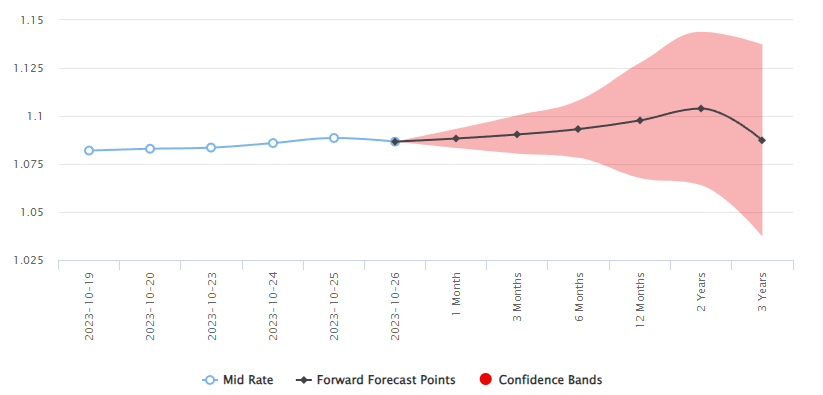
\includegraphics[scale=0.5]{graphs/AUDNZD.png}
\end{figure}

\break

\subsection*{AUD/GBP Forecast}

\noindent The Forward Rate in our analysis, seen in Appendix 2, shows a standard deviation 2.2250, predicting the AUD/GBP rate to be 0.511. This differs slightly from the Commonwealth Bank's (2023) projection of 0.55 GBP by the end of 2023 and Westpac's (2023) prediction of 0.54 GBP for the same period. Meanwhile, Wallet Investor (2023) is more pessimistic, anticipating a rate of around 0.521 as of October 24, 2023. Brexit aftermath and the UK's new trade partnerships could significantly impact GBP. On the other hand, Australia's economic resilience and adaptability to global challenges will determine the AUD's performance. The forecasts vary, but the general sentiment leans towards AUD's depreciation against the GBP.\\

\begin{figure}[h!]
    \centering
    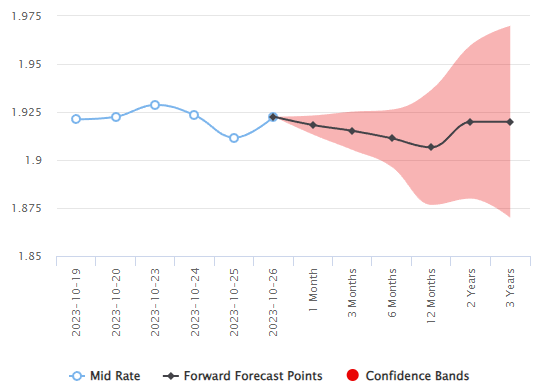
\includegraphics[scale=0.7]{graphs/AUDGBP.png}
\end{figure}

\break

\subsection*{AUD/USD Forecast}

\noindent Given the ongoing momentum indicators, AUD/USD may lean towards a "sell on rallies" position for 2023. The AUD's strength is buoyed by inflation figures and the Reserve Bank of Australia's hawkish stance. According to the Fundamental approach in our analysis in Appendix 3, the predicted rate is 0.644 with a standard deviation of 3.0079. The pair's resistance is at 0.6400, but a break could see it reaching 0.6429. Factors like the RBA's hawkish stance, which contrasts with the US Federal Reserve's expected aggressive rate hikes, will be influential. Australia's global stance, especially its relationship with major economies like China and the US, can significantly affect this pair. Hence, we anticipate the Australian Dollar appreciating against the US Dollar.\\

\subsection*{AUD/JPY Forecast}

\noindent The predominant sentiment for the AUD/JPY pair is bearish for 2023. Following a 15\% rise in 2022, experts believe a long-term decline is on the horizon for the upcoming year. Using the Random Walk model within our analysis seen in Appendix 4, with the lowest deviation at 3.5094, the forecasted rate is 94.38. In contrast, Westpac and NAB predict 96.5 and 87 cents by December 2023, respectively. Therefore, we can say that AUD will still be appreciated over JPY.\\

\subsection*{AUD/EUR Forecast}

\noindent  Fluctuations are anticipated in the Euro to Australian Dollar exchange rate throughout 2023. The Fundamental approach in our analysis, which can be viewed in Appendix 5, with its lowest standard deviation of 2.3865, projects an AUD/EUR rate of 0.5985. According to market pricing, the rate might be around 1.6667 monthly and 1.6684 in three months. The EU's recovery from the pandemic, combined with its geopolitical stance on issues like climate change and trade, can boost the EUR. Australia's trade agreements with EU member countries and its global stance on similar issues will influence the AUD. Hence, the AUD is projected to depreciate against the EUR.\\

\begin{figure}[h!]
    \centering
    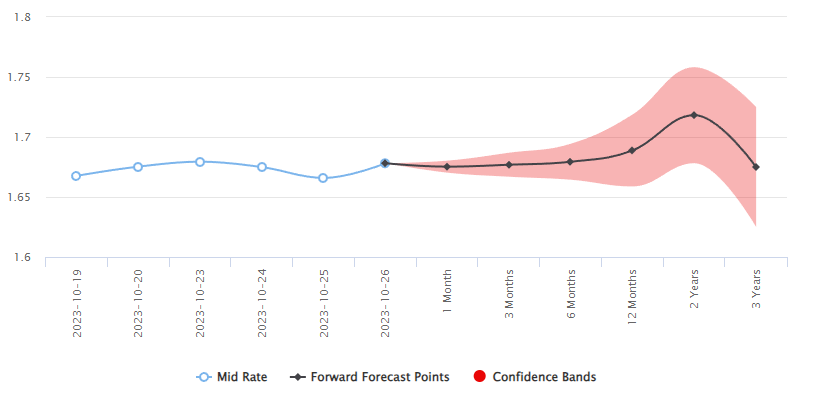
\includegraphics[scale=0.5]{graphs/AUDEUR.png}
\end{figure}

\break

\subsection*{AUD/CAD Forecast}

\noindent In 2023, the Canadian Dollar appreciated 6.42\% against the Australian Dollar, leading to a 6.04\% decrease in the AUD/CAD exchange rate. As per the Fundamental Approach's prediction in Appendix 6, with a deviation of 1.7891, the forecasted rate for AUD/CAD is set at 0.8756. Canada's position as a major oil exporter and its relationship with its North American counterparts, particularly the US, will drive the CAD. Australia's stance on global energy markets will impact the AUD, especially its coal exports and the shift towards renewable energy. Hence, AUD is expected to depreciate against CAD.\\


\noindent Given the diverse forecasts and inherent volatility of currency exchange rates, Firm ABC must judiciously approach its hedging and risk management strategies. By monitoring these rates and using a combination of different hedging techniques, the company can potentially mitigate its exposure to adverse currency movements.\\

\section*{Evaluation of Firm ABC's exposure}
\addcontentsline{toc}{section}{Evaluation of Firm ABC's exposure}

Firm ABC has a widespread international presence, exposing it to many currency-related risks: transactional, translational, and economic. As the world grapples with uncertainties, a proactive approach to these exposures must be taken to ensure the firm's profit margins, liquidity, and overarching strategic goals.\\

\subsection*{Hedging Strategies Explored}

\noindent \textbf{Forward Hedging:}\\
\begin{itemize}
    \item \textbf{Advantages:} This method secures an exchange rate for upcoming transactions, clarifying future cash flows. It is a direct approach that eradicates currency risks.
    \item \textbf{Disadvantages:} Should the market move favourably, Firm ABC misses out. Once settled upon, it lacks flexibility.
    \item \textbf{Overall Impact:} With stable anticipated cash flows, the cost of capital could be reduced due to increased earnings predictability.\\
\end{itemize}

\noindent \textbf{Money Market Hedging (MMH):}\\
\begin{itemize}
    \item \textbf{Advantages:} MMH uses the money market to safeguard against potential foreign exchange liabilities or entitlements. It acts as a buffer against negative currency shifts.
    \item \textbf{Disadvantages:} Compared to forward Hedging, it is more intricate and may sometimes need to be more practical due to fluctuating interest rates across nations.
    \item \textbf{Overall Impact:} MMH offers similar benefits to forward hedging, possibly reducing capital costs.\\
\end{itemize}

\noindent \textbf{Options Hedging:}\\
\begin{itemize}
    \item \textbf{Advantages:} This provides the choice (without obligation) to exchange currency at a predetermined rate, setting a floor and allowing favourable market gains.
    \item \textbf{Disadvantages:} It demands an initial premium, which can be expensive, especially over extended durations.
    \item \textbf{Overall Impact:} While it curtails cash flow volatility, the premium might increase the capital cost.\\
\end{itemize}

\noindent \textbf{No Hedging:}\\
\begin{itemize}
    \item \textbf{Advantages:} The absence of preliminary costs or charges and the ability to fully leverage beneficial market shifts.
    \item \textbf{Disadvantages:} It leaves the company vulnerable to currency risks, potentially leading to considerable fiscal setbacks if rates go south.
    \item \textbf{Overall Impact:} This could heighten the unpredictability of cash flows, possibly augmenting capital costs owing to escalated risks.\\
\end{itemize}

\subsection*{Repercussions on Cost of Capital and Enterprise Value}
\noindent While defending against detrimental currency shifts, Hedging may also curtail the weighted average cost of capital (WACC). With diminished risks, investors may settle for smaller returns, cutting equity costs. Simultaneously, attractive borrowing rates can bring down debt expenditures. This cumulative impact can boost the company's worth.\\

\subsection*{Specific Recommendations for Firm ABC}
\noindent By comparing the most favourable results across different hedging strategies as seen calculated within Appendices 7-13:
\begin{itemize}
    \item NZD Receivables: Forward Contracts heighten outcomes by \$1,787,000.
    \item CAD Receivables: MMH is more fruitful by \$2,961,270.29.
    \item GBP \& EUR Receivables: It is advisable not to hedge.
    \item JPY \& USD Payables: Forward Hedging presents savings, with the USD savings amounting to \$190,006.58.
    \item EUR Payables: Hedging is not beneficial.\\
\end{itemize}

\noindent In juxtaposition with a non-hedging stance:
\begin{itemize}
    \item Forward Contracts heighten the NZD Receivable outcome by \$1,787,000.00, and MMH enhances the CAD Receivable by \$2,961,270.29. However, GBP, EUR Receivables, and EUR Payables fare better unhedged. For JPY and USD Payables, Forward Hedging has savings of \$-2,294.84 and \$190,006.58, respectively.\\
\end{itemize}

\noindent In conclusion, Firm ABC should consider merging both Forward and Options Hedging. The former is apt for specific cash flows, while the latter is more suited for fluctuating ones. This twin-strategy not only offers protection but also flexibility. By actively hedging, Firm ABC can stabilise its future cash flows and alter perceptions about its risk, possibly leading to decreased capital costs. Moreover, shielding against unfavourable currency shifts safeguards firm value, ensuring shareholder wealth remains intact.\\

\section*{Appendices}
\addcontentsline{toc}{section}{Appendices}

\subsection*{Appendix 1- Forecast: NZD}

\begin{figure}[h!]
    \centering
    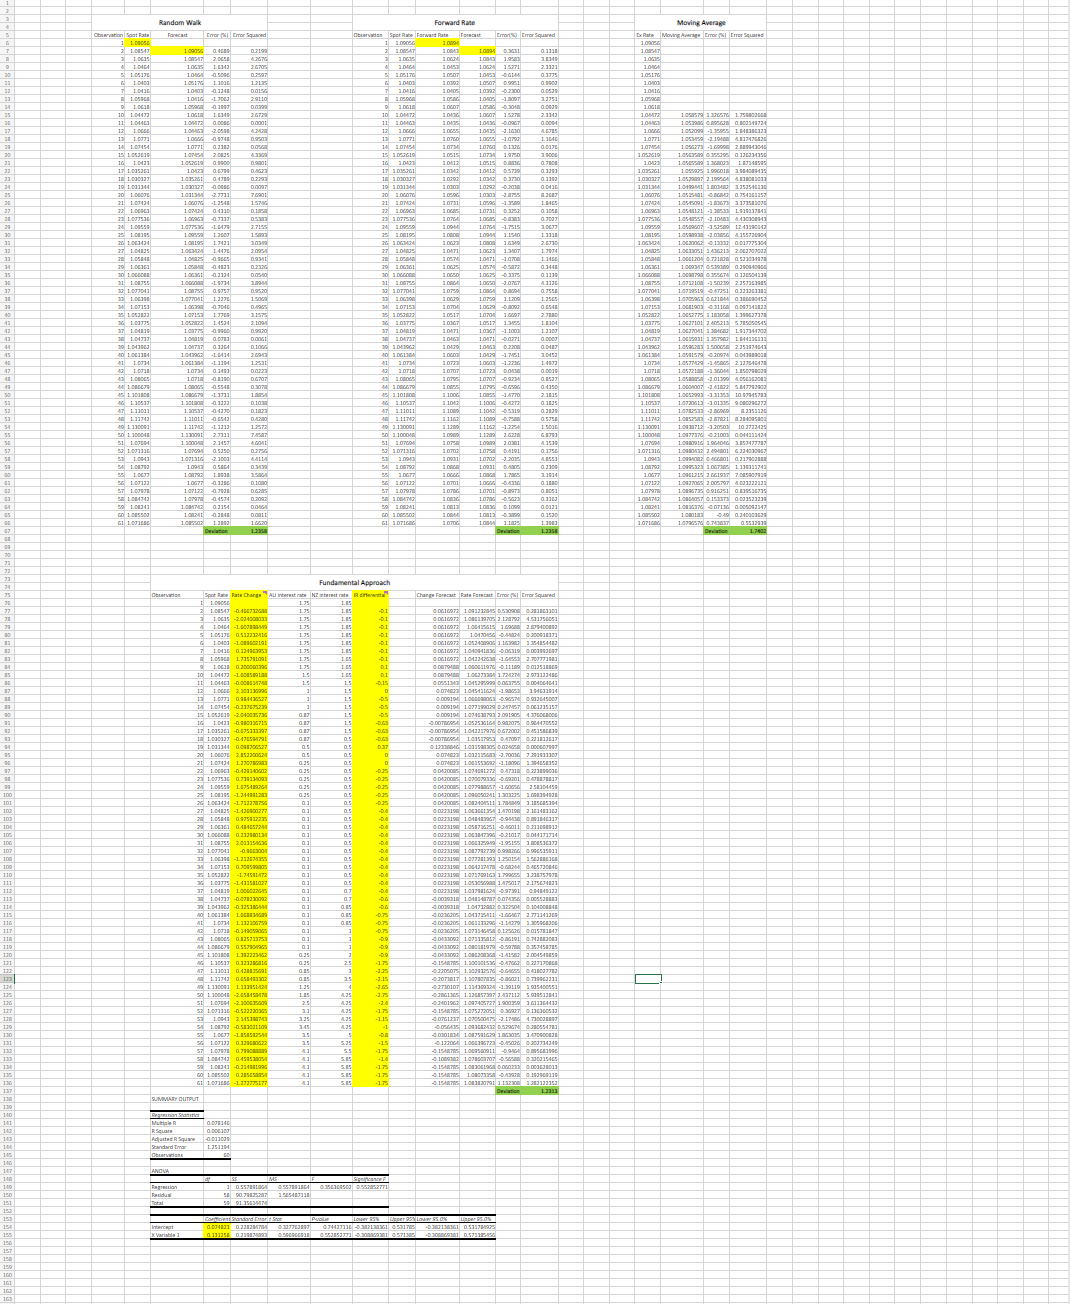
\includegraphics[scale=0.5]{forecasts/NZD.png}
\end{figure}

\break

\subsection*{Appendix 2- Forecast: GBP}

\begin{figure}[h!]
    \centering
    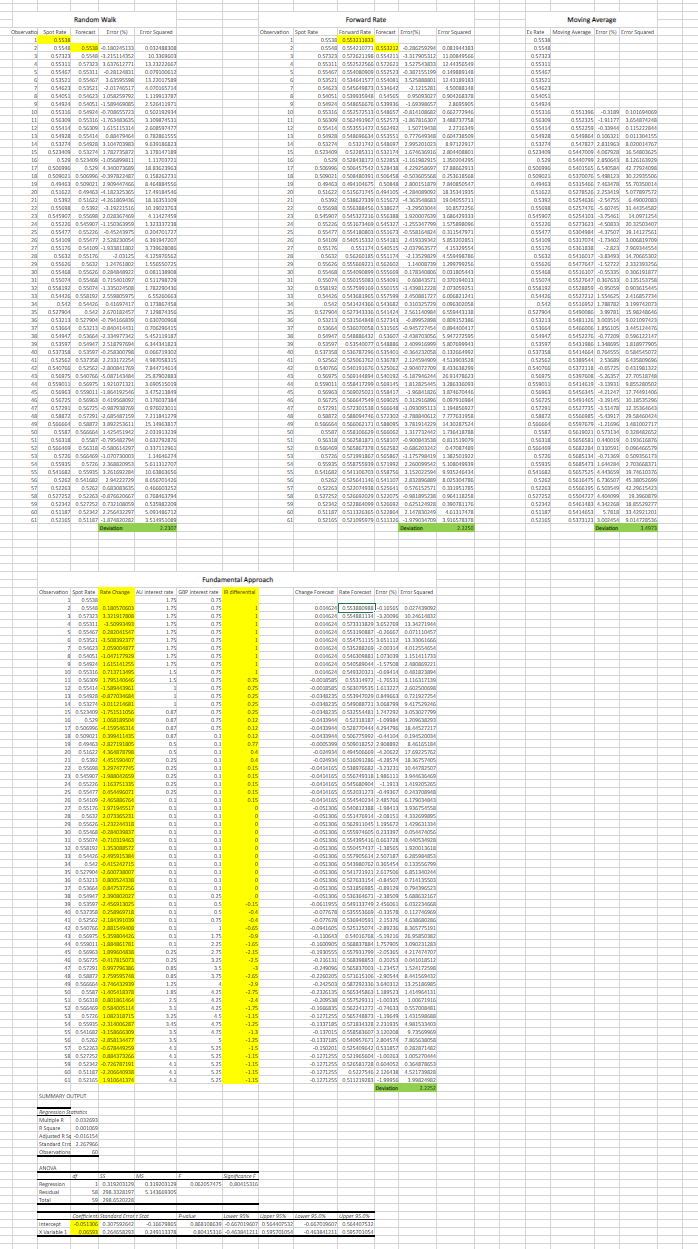
\includegraphics[scale=0.5]{forecasts/GBP.png}
\end{figure}

\break

\subsection*{Appendix 3- Forecast: USD}

\begin{figure}[h!]
    \centering
    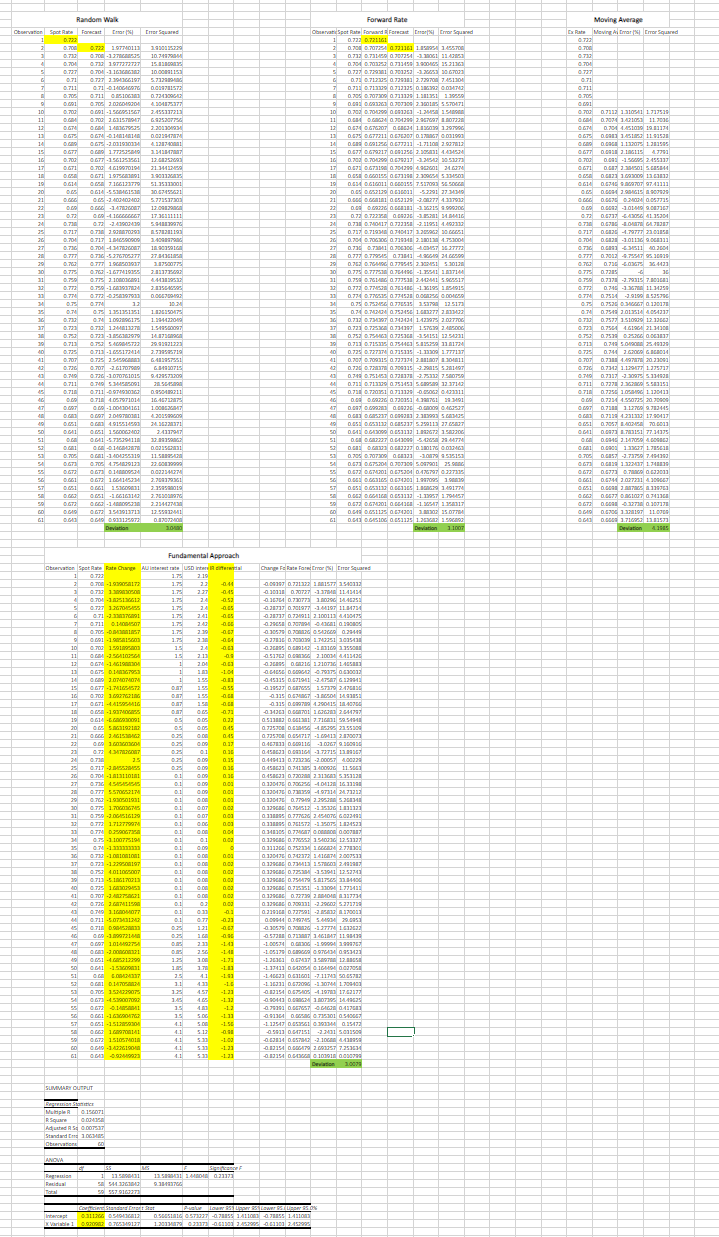
\includegraphics[scale=0.5]{forecasts/USD.png}
\end{figure}

\break

\subsection*{Appendix 4- Forecast: JPY}

\begin{figure}[h!]
    \centering
    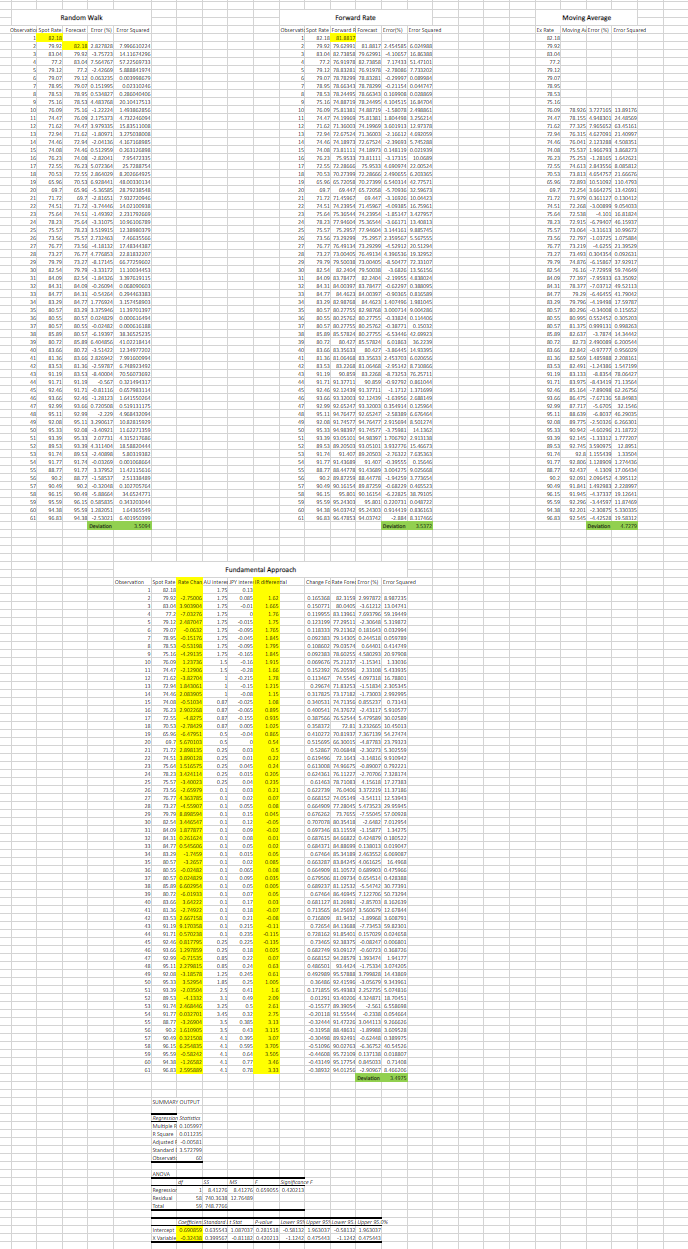
\includegraphics[scale=0.5]{forecasts/JPY.png}
\end{figure}

\break

\subsection*{Appendix 5- Forecast: EUR}

\begin{figure}[h!]
    \centering
    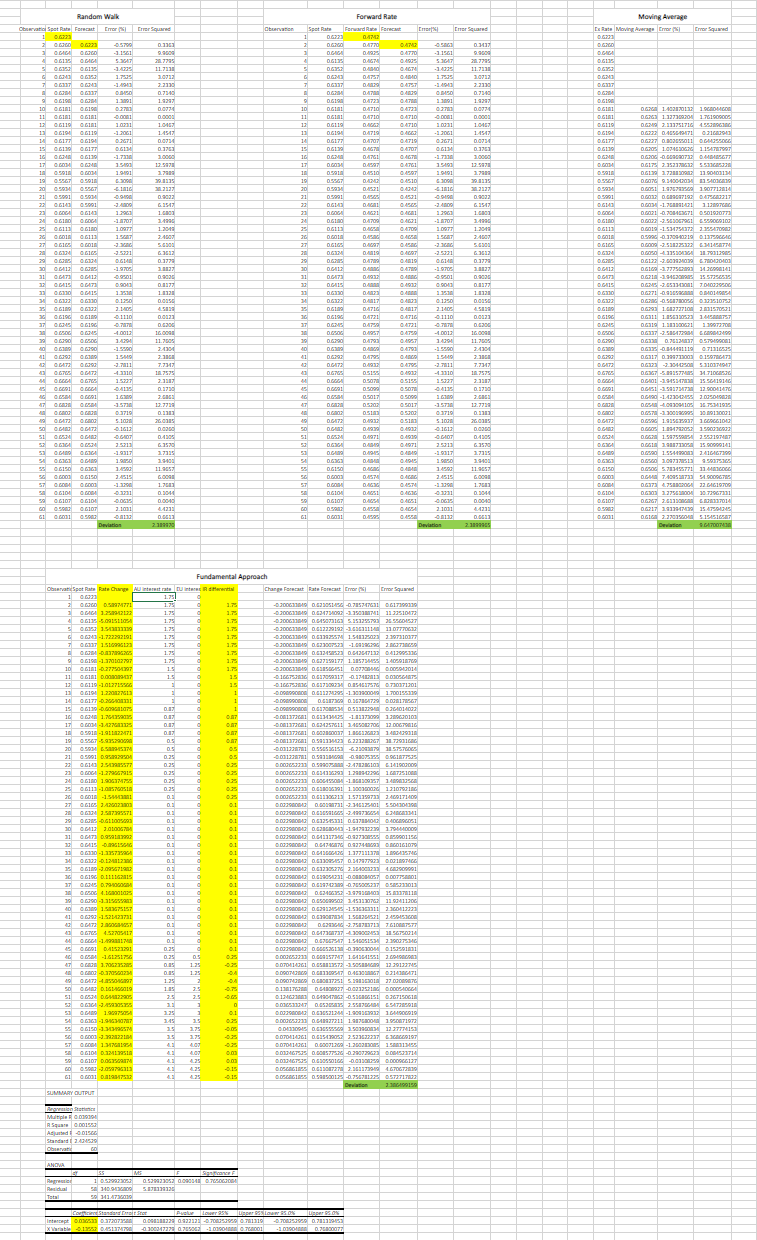
\includegraphics[scale=0.5]{forecasts/EUR.png}
\end{figure}

\break

\subsection*{Appendix 6- Forecast: CAD}

\begin{figure}[h!]
    \centering
    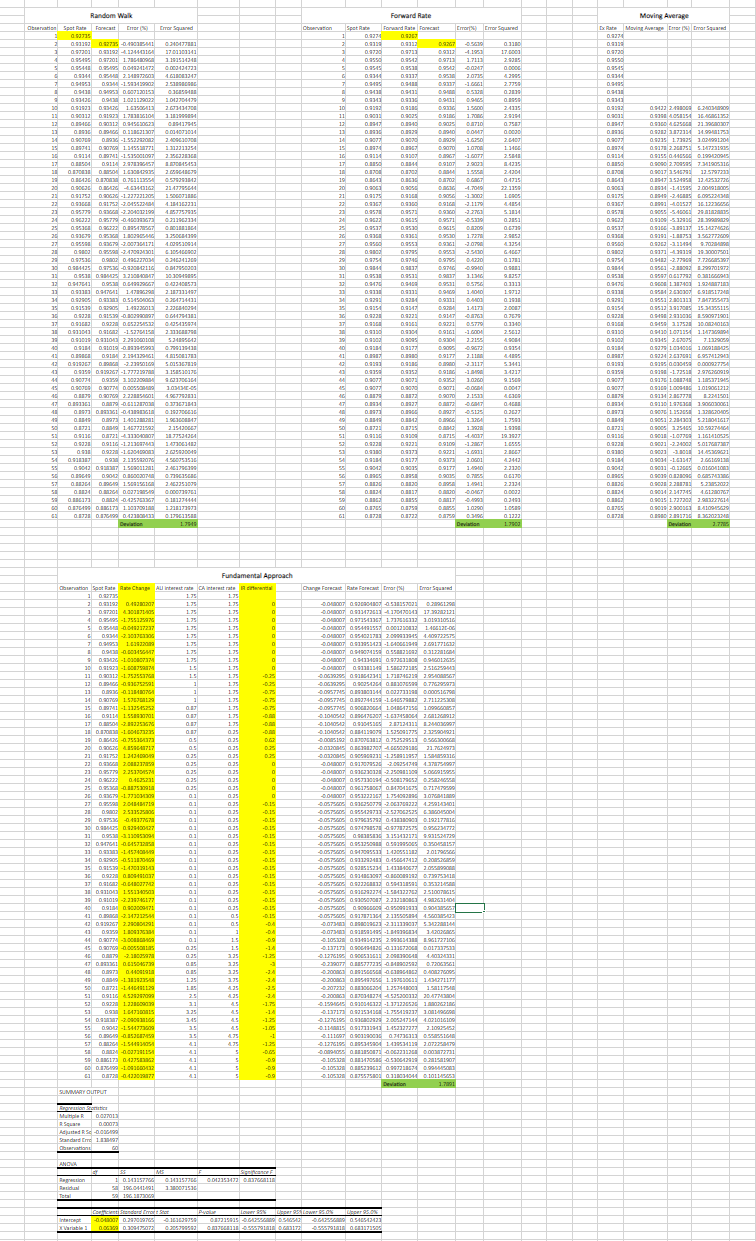
\includegraphics[scale=0.5]{forecasts/CAD.png}
\end{figure}

\subsection*{Appendix 7- Hedge: EUR payable}

\begin{figure}[h!]
    \centering
    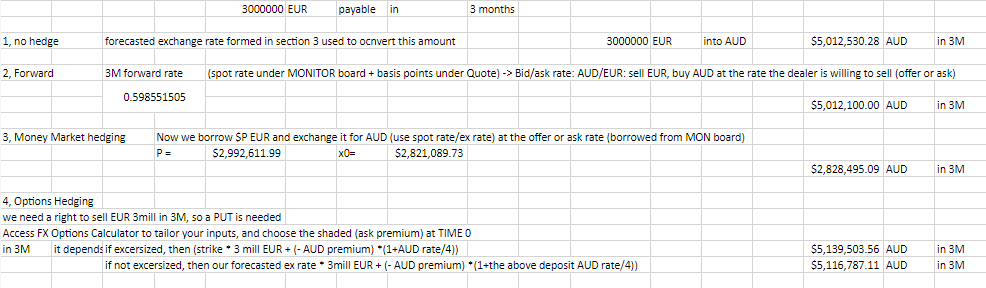
\includegraphics[scale=0.5]{hedge/pay-EUR.png}
\end{figure}

\subsection*{Appendix 8- Hedge: JPY payable}

\begin{figure}[h!]
    \centering
    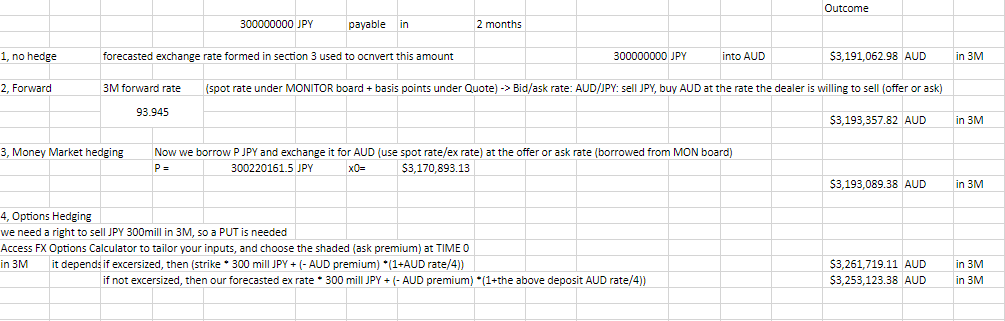
\includegraphics[scale=0.5]{hedge/pay-JPY.png}
\end{figure}

\subsection*{Appendix 9- Hedge: USD payable}

\begin{figure}[h!]
    \centering
    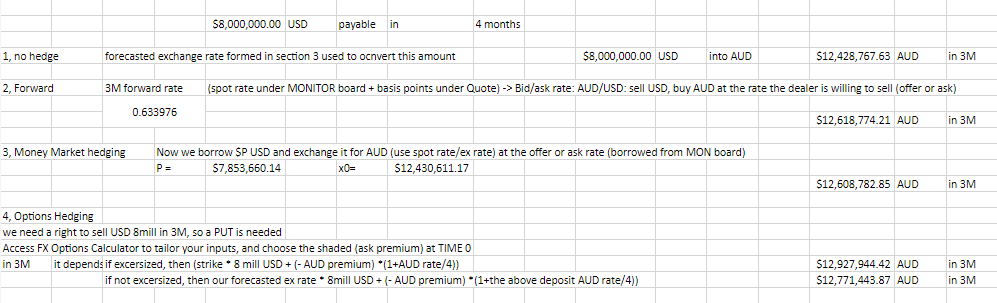
\includegraphics[scale=0.5]{hedge/pay-USD.png}
\end{figure}

\subsection*{Appendix 10- Hedge: CAD receivables}

\begin{figure}[h!]
    \centering
    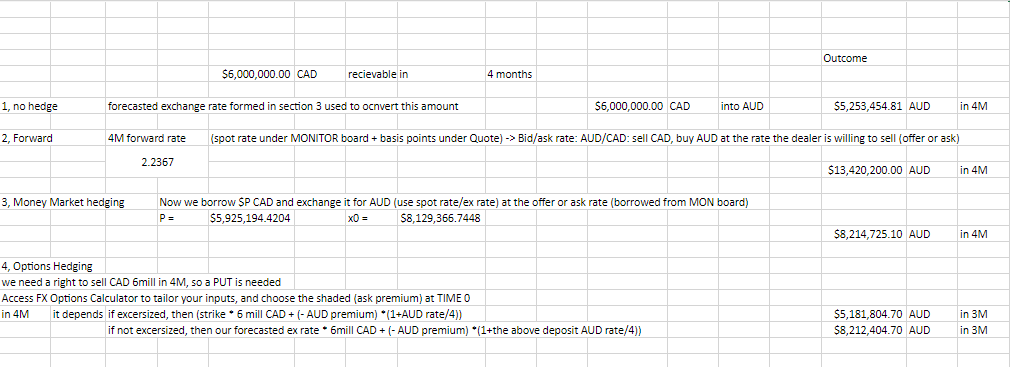
\includegraphics[scale=0.5]{hedge/rec-CAD.png}
\end{figure}

\subsection*{Appendix 11- Hedge: EUR receivable}

\begin{figure}[h!]
    \centering
    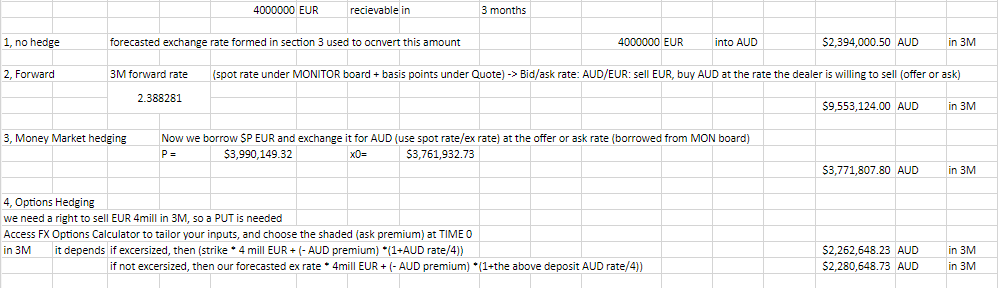
\includegraphics[scale=0.5]{hedge/rec-EUR.png}
\end{figure}

\subsection*{Appendix 12- Hedge: GBP receivable}

\begin{figure}[h!]
    \centering
    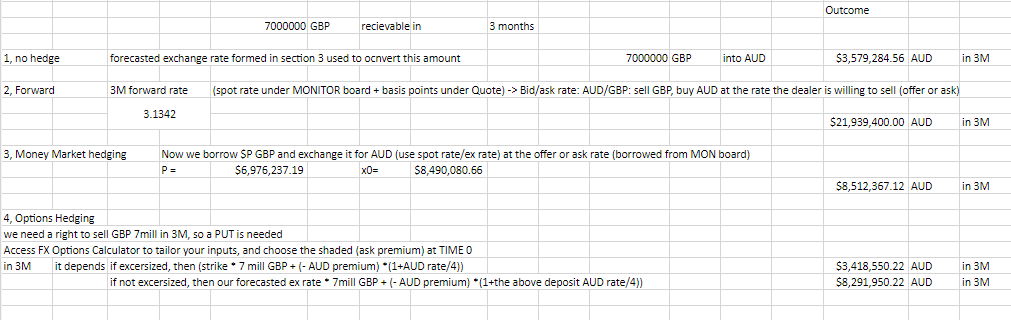
\includegraphics[scale=0.5]{hedge/rec-GBP.png}
\end{figure}

\subsection*{Appendix 13- Hedge: NZD receivable}

\begin{figure}[h!]
    \centering
    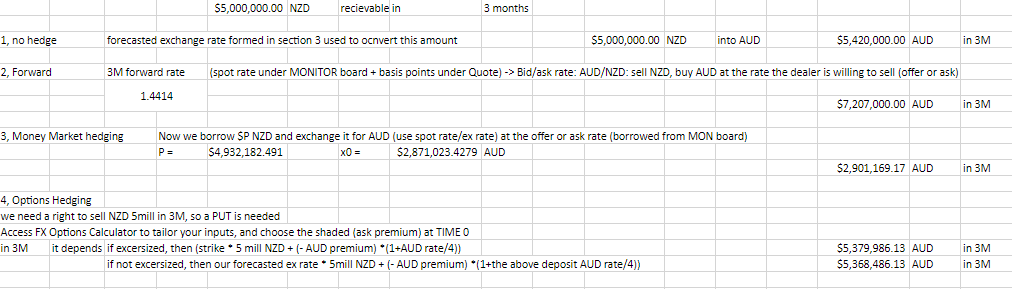
\includegraphics[scale=0.5]{hedge/rec-NZD.png}
\end{figure}

\break


\end{document}  